\section{Database}
In this section we will present the design of our database.
Our design will support the concepts that we have introduced, namely project groups and project group members discussed in~\secref{sec:projectgroups}.

\subsection{Project Group}
A project group must be identifiable by both human and computers.
To make a project group identifiable by humans we give them a short name that must be unique among other project groups.


We decided to give the project group the following attributes. 
\begin{itemize}
	\item An id to identify the group. 
	\item A short name to easily identify the group for humans. 
	\item The full name of the group. 
	\item A timestamp for its creation. 
	\item A set of members. 
\end{itemize}

\subsubsection{Project Group Members}
The set of members denotes a relation between project groups and users and we give it the following attributes: 
\begin{itemize}
	\item An id, which is Moodle convention. \cite{moodledb}.
	\item A reference to the related project group.
	\item A reference to the related user.
	\item A role denoting the type of membership the user has to the group.
	\item A timestamp for its creation.
	\item A timestamp for the last update to the membership. 
\end{itemize}
The database scheme can be seen in~\figref{fig:projectgroupsdb}. 
The user entity is an inbuilt part of Moodle and is not modeled by us. 
\begin{figure}
	\centering
		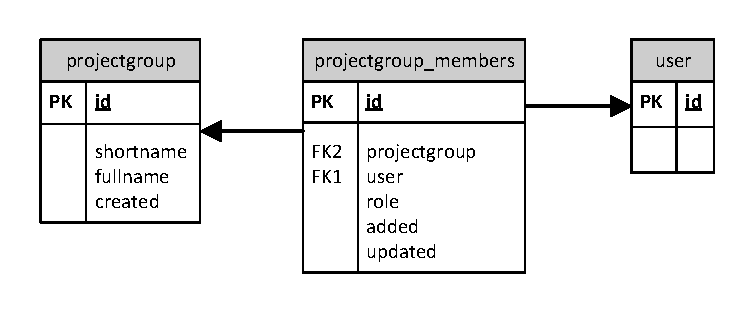
\includegraphics{images/projectgroupsdb.pdf}
	\morscaption{The database scheme of project groups and memberships. The data fields of the user table is omitted for brevity}
	\label{fig:projectgroupsdb}
\end{figure}

%To test the scheme for redundancy we check to see that the scheme conforms to boyce-codd normal form (BCNF). To check this we 

